\documentclass[10pt,twocolumn,letterpaper]{article}
%% Welcome to Overleaf!
%% If this is your first time using LaTeX, it might be worth going through this brief presentation:
%% https://www.overleaf.com/latex/learn/free-online-introduction-to-latex-part-1

%% Researchers have been using LaTeX for decades to typeset their papers, producing beautiful, crisp documents in the process. By learning LaTeX, you are effectively following in their footsteps, and learning a highly valuable skill!

%% The \usepackage commands below can be thought of as analogous to importing libraries into Python, for instance. We've pre-formatted this for you, so you can skip right ahead to the title below.

%% Language and font encodings
\usepackage[spanish,english]{babel}
\usepackage[utf8x]{inputenc}
\usepackage[T1]{fontenc}

%% Sets page size and margins
\usepackage[a4paper,top=3cm,bottom=2cm,left=3cm,right=3cm,marginparwidth=1.75cm]{geometry}

%% Useful packages
\usepackage{amsmath}
\usepackage{graphicx}
\usepackage[colorinlistoftodos]{todonotes}
\usepackage[colorlinks=true, allcolors=blue]{hyperref}
\usepackage[toc,page]{appendix}
%% Title
\title{
		%\vspace{-1in} 	
		\usefont{OT1}{bch}{b}{n}
		\normalfont \normalsize \textsc{Machine Learning class project 2021, Fall} \\ [10pt]
		\huge A comparative study of traditional Machine Learning Models on Seizure Detection and Prediction  \\
}

\usepackage{authblk}

\author[1]{Shivam Bajaj}
\author[1]{Ruochen Kong}


	\affil[1]{\small{Department of Computer Science, Emory University}}

\usepackage{pdfpages}

\begin{document}
\maketitle

\selectlanguage{english}
\begin{abstract}
Most parts of epilepsy care revolve around seizure detection, prediction, and prevention. This paper presents an analysis system for detecting and predicting epileptic seizures from EEG signals. In this study, seven different statistical features are analyzed for their impact and then extracted from each band of the RAW EEG Data, which are the mean value of each channel, Power spectral density(PSD), Frequency Fourier Transform(FFT), Hjorth parameters, Higuchi Fractal Dimension(HFD), Petrosian Fractal Dimension(PFD). To further study these features, metrics are defined based on their influence on models. Next, with the knowledge of the extracted features, a comparative study is proposed by the models of Logistic Regression(LR), SVM's, CS-SVMs, and Multilayer Perceptron(MLP), aiming to discriminate non-seizure signals from seizure signals. In terms of classification accuracy, sensitivity, and specificity, preliminary studies with 99 epileptic events reveal that the suggested methodology is a powerful tool for detecting seizures in epileptic signals. 
\end{abstract} \\ 
\\ 
{\textbf{Keywords} \\
Higuchi Fractual Dimension, Petrosian Fractal Dimension, Logistic Regression, Multilayer Perceptron, SVM}

\section{Introduction}
Seizure is a paroxysmal event caused by abnormal excessive or synchronous neuronal activity in the brain. Abnormal excessive hypersynchronous neuronal activity in the brain often causes a transient occurrence of signs or signals, indicating the occurrence of an epileptic seizure \cite{intro_2}. Epilepsy is a serious neurological disorder with unique characteristics, tending to recurrent seizures\cite{intro_1}. 

According to the World Health Organization\cite{intro_3}, more than 50 million people worldwide suffer from epilepsy with approximately 80 percent of them living in poor countries. By estimating, three out of every four people in these countries with this ailment fail to receive appropriate diagnosis or treatment. 

The most common symptom of epilepsy is when a patient has more than one episode. It causes an abrupt breakdown or unexpected activity in the brain, resulting in an involuntary change in a patient's behavior, sensations, and loss of consciousness for a brief period of time. Seizures can last anywhere from a few seconds to a few minutes and can occur at any time without warning. This can result in significant physical injuries such as fractures, burns, and even death, as well as mental diseases such as depression\cite{Unpredictability}.

\section{A paradigm for detecting seizures}
\begin{figure*}[h]
  \centering
  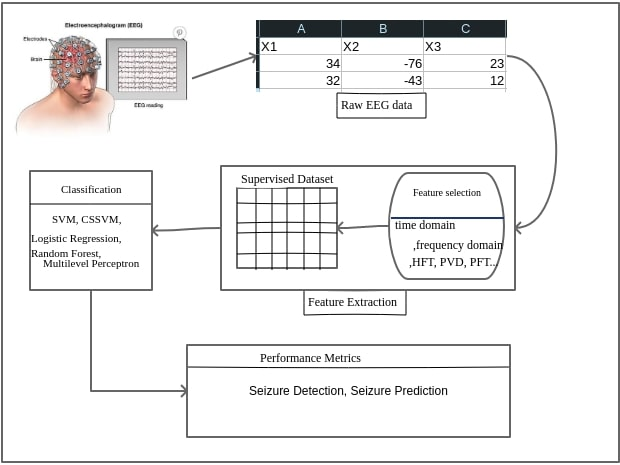
\includegraphics[width=\textwidth,height=10cm]{fff.jpg}
  \caption{Implementation for identifying epileptic seizures. This describes the basic steps for collecting the dataset using an EEG medium, displaying raw EEG signals, converting EEG signals to a two-dimensional table, feature selection, preparing the dataset with seizure (ictal) and non-seizure (interictal), applying machine learning classifiers and seizure detection, and other related tasks. }
\end{figure*}

In this section, we offer a visual framework of the model utilized for seizure identification from an EEG seizure dataset, as seen in Figure 1. There are four main steps in the procedure: Data collection, data preparation, machine learning classification, and performance evaluation. 
\subsection{Data Collection}
For the seizure identification and prediction sections, the RAW EEG data used were from a competition sponsored by the University of Pennsylvania, the National Institutes of Health (NINDS), the Epilepsy Foundation, the American Epilepsy Society, and the Mayo Clinic Dataset. The data was arranged into matrices of EEG sample data by electrode and time (row x column). The recording time for each electrode was set to one second. Latency, which indicates the interval in seconds between the start data point in the data segment and the expert-marked seizure onset, and sampling frequency, which represents the number of data samples presented in one second of EEG data, were also included in the data. These datasets were collected as EEG samples from several Patients and Canines suffering from Epilepsy\cite{Competition}.

\subsection{Feature Extraction}
These RAW EEG data cannot be directly statistically assessed due to the lack of valuable information.
Thus, to address this problem, a collection of statistical traits is extracted to help produce more noteworthy outcomes. 
\subsubsection{Latency}
Latency, as a part of the raw dataset, would possibly relate to the magnitudes of signals and hence influent the detection or prediction results, so it is sorted as the first feature.

\subsubsection{Mean}
The mean is a basic but commonly used statistical feature, which is calculated by dividing the sum of data by the number. In this project, a mean value is obtained from each electrode channel and regularized before being stored as a feature. Let ${\bf x}$ represents the vector of mean values from all chanels, $\mu$ as its mean, and $\sigma$ as its standard deviation, then the final feature to store is calculated as
\begin{equation}
{\bf x'} = \frac{{\bf x}-\mu}{\sigma}
\end{equation}
\subsubsection{Max-Min}
The maximum and minmum are also fundamental statistical features, but instead of using them directly, the max-min value is considered due to the concerning of the number of overal features. These values are also normalized (eq. 1) and then stored.

\subsubsection{Power spectral density (PSD)}
To start with, a set of frequency bands is defined as 0.1-4Hz (delta), 4-8Hz (theta), 8-12Hz(alpha), 12-30Hz(beta), 30-70Hz(low-gamma), and 70-180Hz(high-gamma)\cite{bands}, which is determined by frequency fourier transfor. The chosen bands are widely accepted and used. Then PSD is calculated under each band for each channel. Let ${\bf x}$ denote the time series in one channel, and let $X$ denote the fast fourier transform of ${\bf x}$, then PSD for the $i$th band is calculated as 
\begin{equation}
PSD_i = \sum X_j \text{  for all } X_j \in \text{band}_i
\end{equation} 
In this project, these values are obtained by with the package PyEEG \cite{pyeeg}.
\subsubsection{Fast Fourier Transform (FFT)}
An FFT converts a time series data, represented as amplitudes against time, to data in the frequency domain. This method is commonly used for analyzing EEG dataset.
\subsubsection{Hjorth parameters}
Hjorth's parameters are introduced and defined in this section\cite{HjorthParam}.
\subparagraph{Hjorth Activity}
The transmit power, or variance, of a time function, is denoted by the Hjorth activity parameter. This can illustrate the frequency domain surface of a power spectrum. 

The following equation explains this:
\begin{equation*}
\text{Hjorth Activity} ={\text{var}} (y(t)).
\end{equation*}

\paragraph{}The signal is represented by $y(t)$.

\subparagraph{Hjorth Mobility}
The power spectrum's mean frequency or proportion of standard deviation is represented by the mobility parameter. This is equal to the square root of the variance of the signal's first derivative $y(t)$ divided by the variance of the signal $y(t)$. 

The following equation explains this:\hfill \break \hfill \break \begin{equation}
\text { Mobility }=\sqrt{\frac{\operatorname{var}\left(\frac{d y(t)}{d t}\right)}{\operatorname{var}(y(t))}} .
\end{equation}
\paragraph{}The signal is represented by $y(t)$.
\paragraph{}In other words, the square root of the ratio between the Hjorth Activity of the time derivative of the frequency signal $y(t)$ and the Hjorth Activity of the frequency response $y(t)$ gives the Hjorth mobility of a vibration signal $y(t)$ \cite{HjorthMob}. 

\subparagraph{Hjorth Complexity}
The frequency change is expressed by the Complexity parameter. The parameter analyzes the signal's resemblance to a pure sine wave, and if the signal is more similar, the value converges to $1$. 

The following equation explains this:
\begin{equation}
\text { Complexity }=\frac{\text { Mobility }\left(\frac{d y(t)}{d t}\right)}{\text { Mobility }(y(t))}
\end{equation}

\paragraph{}Complexity gives an estimate of the bandwidth of the signal, which indicates the similarity of the shape of the signal to a pure sinusoidal wave\cite{HjorthMob}.

\paragraph{}The PyEEG\cite{pyeeg} package is used to obtain the Hjorth mobility and complexity.

\subsubsection{Higuchi Fractal Dimension (HFD)}
Higuchi fractal dimension is a time-domain feature that is extracted from time series and widely applied to classify waves. The Higuchi method is an algorithm for calculating this value. In this method, the original time series data ${\bf x} = [x_1,x_2,\ldots,x_N]$ ìs seperated into $k$ new series. For $m\in[1,k]$, the $m$th new series ${\bf x}_m = \{x_i: i =_{mod\ k} m\}$. Then for each new series, the length $L_m(k)$ is defined as:
\begin{equation}
L_m(k) = \frac{N-1}{|{\bf x}_m|k^2}\sum_{i=1}|x_{m,i} - x_{m,i-1}|.
\end{equation}
Then $L(k)$ is calculated as the average of $L_m(k)$, which is represented
\begin{equation}
L(k) = \frac{1}{k}\sum^m_{i=1} L_i(k)
\end{equation}
Finally, HFD is defined as the slope of the line that best fits $\{ln(k),ln(L(k))\}$. In this project, HFD is calculated with PyEEG \cite{pyeeg}.

\subsubsection{Petrosian Fractal Dimension (PFD)}
Let $N$ denote the length of time series, and $H_\delta$ denote the number of occurrences that the sign of the signal derivative is reversed, then PFD is defined as \cite{pfd}:
\begin{equation}
PDF = \frac{log_{10}(N)}{log_{10}(N) + log_{10}(\frac{N}{N+0.4N})}.
\end{equation}
The lowest value of PDF is $1$ which occurs when no such reversing of the sign exists.

\subsection{Models}
After browsing the prepared dataset, an obvious property can be drawn, namely the imbalance in the numbers between two classes. With the goal to alleviate the impact of this imbalance, a cost-sensitive SVM (CS-SVM) can be considered. In this model, several parameters contribute to amplifying the importance of a class, thus partially solving the imbalance. Hence, according to the paper ``Seizure Prediction with Spectral Power of EEG using a cost-sensitive support vector machine'', Y. Park et al. (2011)\cite{cs-svm} applied CS-SVM to their dataset and resulted in a reliably highly-performed model. The SVM and CS-SVM will be described in the following sections.

\subsubsection{SVM}
Support vector machines, first developed in 1992 \cite{svm}, are supervised learning models that were originally used to linearly distinguish two categories. After using a non-linear kernel, these models can also apply to a non-linear classificaion\cite{kernel}. The kernel is defined as $K(x,x')=\phi(x)\cdot\phi(x')$. Hence the loss function is:
\begin{equation*}
\mathcal{L} = \frac{1}{2}||w||^2 
+ C\sum_{i=1}^{N}max\{0, 1-y_i(w^T\phi({\bf x}_i)+b)\}
\end{equation*}
In this project, $C = 1$ is fixed and a radial basis function (rdf) kernel is used, which is defined as $K(x,x')=exp(-\gamma||x-x'||^2)$, along with $\gamma = \frac{1}{p\cdot var(X)}$ where p represents the number of features. 

\subsubsection{CS-SVM}
Cost-sensitive support vector machines are differently implemented. The CS-SVM used in this project is defined with the loss function:
\begin{align*}
\mathcal{L} &= \frac{1}{2}||w||^2\\
 &+ C\sum_{i=1}^{N} max\{0, 1-r_k\cdot y_{i,k}(w^T\phi(x_k)+b)\}
\end{align*}
with $k = \{+1,-1\}$ and $r_k$ represents weight for each class. In this project, $r_{+1} = 1$ is fixed, and the smaller the $r_{-1}$ the less weighted loss of data in class -1. As previously mentioned, the datasets used in this project are highly imbalanced, so without these parameters, the overall loss of the class with more data points would be added up to much higher than the class with fewer data points, even with the same average loss. Thus, the loss should be balanced to allow the model to learn more for the class with fewer data points. In this part, $r_{-1}$ and $C$, which inversely represent the strength of regularization, are determined through 5 nested fold cross-validation with the optimal AUC value.

\subsubsection{Logistic Regression}

Logistic regression is a type of functional classification model that is based on the number of attribute values and the categorized prognosis of the output. Logistic regression was employed in the first set of studies using classification algorithms. The classification yields a value between [0, 1], which is understood as the probability $h(x)$ that the class of x is 1. The sigmoid function used in logistic regression and is defined as:

$$
f(z)=\frac{1}{1+e^{-z}}
$$
where $z$ is of the form: $z=\beta_{0}+\beta_{1} x_{1}+\beta_{2} x_{2}+\ldots+\beta_{n} x_{n}$, $\beta_{0}$ is the intercept and $\beta_{1} , \beta_{2} , ... , \beta_{n}$ are coefficients of the respective $x_{1}, x_{2},..., x_{n}$. A binary variable in this project is limited to values of 1 and 0, with 1 indicating the occurrence of a seizure (ictal) and 0 indicating the opposite(interictal). The independent variables may be discrete or continuous or a combination of both. Logistic Regression has fewer restrictions, such as not assuming linearity in the connection between the independent variables and the response variable. Logistic Regression calculates changes in the reaction variable's logarithm of odds. The regressed relationship between the response and exogenous variables is not linear because the logarithm of odds is linearly connected to the explanatory variables. The probability of occurrence of an event as a function of the explanatory variables is nonlinear as derived as follows\cite{Logisticr} : 

\begin{equation}
P_{1}(x)=\frac{1}{1+\mathrm{e}^{-\operatorname{logit}\left(P_{1}(x)\right)}}=\frac{1}{1+\mathrm{e}^{-\beta_{0}+\sum_{i=1}^{n} \beta_{i} x_{i}}}
\end{equation}

Logistic Regression forces the probability values to lie between 0 and 1, as shown in the above equation as the RHS, approaches -$\infty$, the value of P1->0 and, when the RHS, approaches +$\infty$, the value of P1->1. To understand and evaluate the coefficients of $\beta_{1} , \beta_{2} , ... , \beta_{n}$ in the Logistic Regression sigmoid function, we used the maximum log likelihood estimation(MLE). 

\subsubsection{Artificial Neural Networks}
In the realm of machine learning for neurosciences, learning with artificial neural networks has emerged as a radically significant framework. Artificial Neural Networks (ANNs) are a type of artificial neural network made up of interdependent processing units that reflectively imitate the structure and objectives of the biological nervous system. ANNs learn by using unique training algorithms based on rules that are thought to imitate the acquisition and integration of biological systems \cite{Logisticr}. The MultiLevel Perceptron Neural Network (MLPNN) will be used to develop classifiers in this study since it is relevant to the application being explored. 

A neural network's architecture may have a superficial input layer that picks up the inputs and an output layer that contains the solution to the problem. Between these two layers, two or more hidden layers process the incoming data and create satisfactory approximations for linear problems. The most crucial challenge with MLPNN models is determining the approximate number of hidden layers to be implemented to get reliable results. Unlike the input and output layers, the number of hidden layers is usually unknown from the outset. These buried layers contain a network of interconnected artificial neurons or nodes. They tend to learn from the data in the input layer and generate accurate estimates based on their knowledge. The data from the input layer is represented as activation values, with a number assigned to each node; the higher the number, the stronger the activation. This data is subsequently disseminated throughout the network. The output nodes then reflect the input to the outside world prudently.

Another significant problem in developing an ANN-based model is estimating the number of nodes each hidden layer contains. A network with too few hidden nodes may be incapable of making sense of the incoming data, resulting in erroneous patterns. In contrast, due to over-parameterization, a network with too many hidden nodes will cause the model to follow the noise in the data. Increasing the number of hidden layers can change the model's time and spatial complexity. As a result, we may infer that trial and error is the most efficient method of determining the number of hidden nodes and layers.

The MLPNN model used in this study has two hidden layers, the first of which had 13 nodes and the second of which had 6. A backpropagation training technique was employed as the training algorithm\cite{backpro}.  


\section{Validation Metrics}
\paragraph{}The first and most important validation is the 5 nested fold cross-validation. During this process, the ROC and AUC can be calculated for the model. Hence, for the CS-SVM model, the AUC value of each $C$,$r_{-1}$ pair can be calculated. The optimal $C$,$r_{-1}$ are then determined by the maximum AUC value. 
\paragraph{}Next comes the Confusion matrix, which is defined as:
\begin{table}[h]
\begin{tabular}{lllll}
          & predicted -1           & predicted +1             \\
actual -1 & \multicolumn{1}{c}{TN} & \multicolumn{1}{c}{FP}   \\
actual +1 & \multicolumn{1}{c}{FN} & \multicolumn{1}{c}{TP}   	
\end{tabular}
\end{table}
\paragraph{}Instead of representing this matrix directly, the graph used in this project is the Confusion matrix divided by the number of data points, so the resulting matrix is represented as the percentage.
\paragraph{} This matrix is also used to calculate accuracy, sensitivity and F1, as:
\begin{align*}
\text{ACC} &= \frac{\text{TP}+\text{TN}}{\text{TP}+\text{TN}+\text{FP}+\text{FN}}\\
\text{Sensitivity} &= \frac{\text{TP}}{\text{TP}+\text{FN}}\\
\text{F1} &= \frac{2\text{TP}}{2\text{TP}+\text{FP}+\text{FN}}
\end{align*}
In this project, the accuracy does not reliably represent the performance of a model, because in most dataset the ratio between ictal to interictal, or preictal to interictal, is about 1:9 that even randomly assigning would result in high accuracy.



\section{Results}

\begin{figure*}[h]
  \centering
  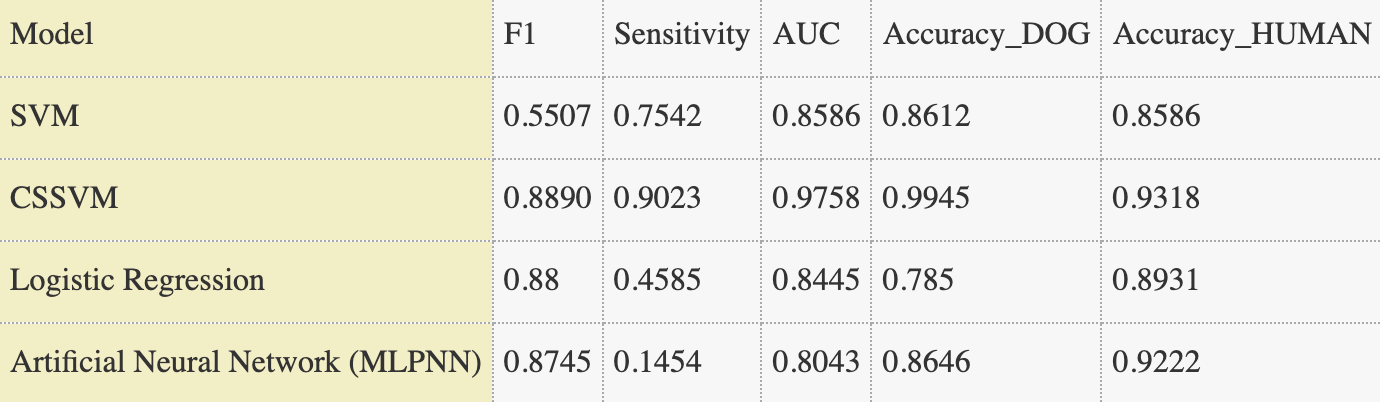
\includegraphics[width=\textwidth,height=4cm]{fwe.png}
  \caption{Summary statistics comparing the different scores achieved by different models. Please note, the features selected for all the models were the same. }
\end{figure*}
Summary results for both detection and prediction and for all patients and canines are shown in Figure 2 and an in-depth explanation of the same is shown in Appendices.


\subsection{SVM \& CS-SVM}
\paragraph{} As the baseline, in detection, the SVM has average accuracy at $86.0\%$, sensitivity at $75.4\%$, and F1-score at $55.1\%$. These values are all relatively lower than the CS-SVM model, which are $95.3\%$, $90.2\%$, and $88.9\%$. In prediction, the SVM has average accuracy at $78.8\%$, sensitivity at $4.5\%$, and F1-score at $5.1\%$, while these values for the CS-SVM model are $72.2\%$, $77.6\%$, and $38.9\%$. 
\paragraph{}Both models perform better in the dataset of canines, which is probably because more data points are collected for canines. For CS-SVM with the task of detection, an outlier occurs at patient 4 with accuray only about $50\%$. This problem might be due to the lack of data points. Specifically, 210 data points are collected but 865 features are extracted. A principal component analysis (PCA) would solce this problem that will achive in future research. 
\paragraph{}In detection, the CS-SVM performs generally better than SVM, but different in prediction task. Comparing CS-SVM to SVM in prediction task, although the accuracy drops a little, sensitivity and F1 increase significantly, especially for the sensitivity.The increase of sensitivity can be understood as the CS-SVM cares more about the ictal, or preictal, data rather than the interictal data. This more attention meets the overall goal of seizure detection or prediction because the occurrence of seizures is more important than normal conditions.
\paragraph{}When browsing through the Confusion matrix generated by SVM, a problem can be obviously noticed that the model labeled almost every data points into ``-1''. This disability of learning indicates the problem of features extraction on prediction datasets. The raw data of prediction differently consists with the detection, but the same methods were used for feature extraction which results in the inseparable of two categories.
\paragraph{}The matrix of AUC values for determing the optimal $C$, $r_{-1}$ pairs also shows a specific pattern. The $r_{-1}$ value optimized at $\frac{N_{+1}}{N_{both}}$ frequently, which confirms the previous guess that the imbalance will cause a problem. For the $C$ values, the larger the $C$ corresponding to the higher the performance, namely the increase of regularization strength will not improve the performance for these datasets.

\subsection{Logistic Regression \& ANNs}
\paragraph{} For developing the Logistic Regression and Artificial Neural Network, we split the data into 3 parts; 80$\%$ of the data was used for the training, 10$\%$ for testing, and 10$\%$ for validation. Logistic Regression, averaged an 83.90$\%$ accuracy, 88$\%$ f1 score, 45.8$\%$ sensitivity, and displayed an AUC score of 0.74. The ANNs on the other hand performed exceptionally well. They displayed an average accuracy of 86.46$\%$ an F1 score of 87.45$\%$, sensitivity of 14.45$\%$, and an average AUC score of 0.8043. The AUC score for classifiers is given in Figure 2. The AUC score achieved by the MLPNN model is far superior to the Logistic Regression score. This proves that the MLPNN classifier tends to work better than the Logistic regression model. 

Although we could not achieve a satisfactory sensitivity score, this was mainly because the model, was very biased towards interictal data. The neural network diagnostic system's testing performance was designed to be accurate, and we believe that if it is perfected, it will be useful in clinical investigations. This tool offers fairness to EEG signal evaluation, and its autonomous nature makes it simple to implement in medical research.   By studying the EEG data with real-time implementation, a "black box" device that may be built as a consequence of this work might offer input to neurologists for the categorization of the EEG signals fast and precisely.



\section{Research challenges in seizure detection}
One difficulty is the lack of background knowledge, which causes us to spend time investigating reasonable features. Even after spending such an amount of time, the optimal way to extract features from the prediction datasets remains a struggle. Selecting the kernel of SVM also causes a problem, because the optimal one is hard to be determined. Hence, we create models for each individual dataset, but the relation between them is unable to conclude and thus causing difficulties in creating a more general model.

\section*{Conclusions} In this paper, four approaches to developing classifiers for detecting and predicting EEG seizures in dogs and humans were discussed. One approach is based on the traditional Support Vector Machines model that was found to almost failing in all datasets. We suspect that this might be due to the limited generalization of the features extracted. CS-SVM, on the other hand, tends to have performed better than SVM but also faces problems in the prediction task. For this task, to increase the sensitivity, CS-SVM sacrifices the accuracy, indicating the inseparability of data points. The Logistic Regression model performed predominantly well on the detection datasets. Although the MLPNN classifier aided to be more accurate, there still seems to be some misclassifications. Compared to the Logistic Regression, MLPNN include their robustness to noisy data (with outliers) which can severely hamper many traditional statistical methods. MLPNN required deciding the number of hidden layers and number of hidden neurons to fit each on each hidden layer, the number of iterating cycles and the choice of the activation function, selection of optimal learning rate, and other parameters pertaining to the convergence of the solution. One advantage that MLPNN has over the other classifiers is that MLPNN can quickly be developed, and retrained if implemented in the hardware of EEG systems. Further study will take to continuously find the optimal method of feature extraction.

\section*{Authors' Contributions}
R.K. and S.B. contributed to the feature extraction of the project, as well as the presentations and the final version of the report. R.K. designed and analyzed the model of SVM and CS-SVM. S.B. designed and analyzed the model of LR and ANN.

\begin{thebibliography}{9}

\bibitem{intro_2}Fisher RS, van Emde Boas W, Blume W, Elger C, Genton P, Lee P, Engel J Jr. Epileptic seizures and epilepsy: definitions proposed by the International League Against Epilepsy (ILAE) and the International Bureau for Epilepsy (IBE). Epilepsia. 2005 Apr;46(4):470-2. doi: 10.1111/j.0013-9580.2005.66104.x. PMID: 15816939.
\bibitem{HjorthParam} Bo Hjorth,
EEG analysis based on time domain properties,
Electroencephalography and Clinical Neurophysiology,
Volume 29, Issue 3,
1970,
Pages 306-310,
ISSN 0013-4694,
https://doi.org/10.1016/0013-4694(70)90143-4.
\bibitem{intro_1} World Health Organization. (2006). Neurological disorders: public health challenges. World Health Organization.
\bibitem{intro_3}World Health Organization. Mental Health Action Plan (WHO) 2013-2020.
\bibitem{Competition} Benjamin H. Brinkmann, Joost Wagenaar, Drew Abbot, Phillip Adkins, Simone C. Bosshard, Min Chen, Quang M. Tieng, Jialune He, F. J. Muñoz-Almaraz, Paloma Botella-Rocamora, Juan Pardo, Francisco Zamora-Martinez, Michael Hills, Wei Wu, Iryna Korshunova, Will Cukierski, Charles Vite, Edward E. Patterson, Brian Litt, Gregory A. Worrell, Crowdsourcing reproducible seizure forecasting in human and canine epilepsy, Brain, Volume 139, Issue 6, June 2016, Pages 1713–1722, https://doi.org/10.1093/brain/aww045
\bibitem{bands}Howbert JJ, Patterson EE, Stead SM, Brinkmann B, Vasoli V, Crepeau D, Vite CH, Sturges B, Ruedebusch V, Mavoori J, Leyde K, Sheffield WD, Litt B, Worrell GA. Forecasting seizures in dogs with naturally occurring epilepsy. PLoS One. 2014 Jan 8;9(1):e81920. doi: 10.1371/journal.pone.0081920. PMID: 24416133; PMCID: PMC3885383.
\bibitem{pyeeg}Forrest Sheng Bao, Xin Liu, Christina Zhang, "PyEEG: An Open Source Python Module for EEG/MEG Feature Extraction", Computational Intelligence and Neuroscience, vol. 2011, Article ID 406391, 7 pages, 2011. https://doi.org/10.1155/2011/406391
\bibitem{HjorthMob}Marco Cocconcelli, Matteo Strozzi, Jacopo Cavalaglio Camargo Molano, Riccardo Rubini,
Detectivity: A combination of Hjorth’s parameters for condition monitoring of ball bearings,
Mechanical Systems and Signal Processing,
Volume 164,
2022,
108247,
ISSN 0888-3270,
https://doi.org/10.1016/j.ymssp.2021.108247. 
\bibitem{pfd}A. Petrosian, "Kolmogorov complexity of finite sequences and recognition of different preictal EEG patterns," Proceedings Eighth IEEE Symposium on Computer-Based Medical Systems, 1995, pp. 212-217, doi: 10.1109/CBMS.1995.465426.
\bibitem{cs-svm} Park Y, Luo L, Parhi KK, Netoff T. Seizure prediction with spectral power of EEG using cost-sensitive support vector machines. Epilepsia. 2011 Oct;52(10):1761-70. doi: 10.1111/j.1528-1167.2011.03138.x. Epub 2011 Jun 21. PMID: 21692794
\bibitem{svm} Boser, B. E., Guyon, I. M., \& Vapnik, V. N. A training algorithm for optimal margin classifiers. In Proceedings of the 5th Annual ACM Workshop on Computational Learning Theory (pp. 144-152).
\bibitem{kernel} Thomas Hofmann, Bernhard Schölkopf, Alexander J. Smola "Kernel methods in machine learning," The Annals of Statistics, Ann. Statist. 36(3), 1171-1220, (June 2008)
\bibitem{Unpredictability} Schulze-Bonhage, A. and Kühn, A. (2008). Unpredictability of Seizures and the Burden of Epilepsy. In Seizure Prediction in Epilepsy (eds B. Schelter, J. Timmer and A. Schulze-Bonhage). https://doi.org/10.1002/9783527625192.ch1

\bibitem{Logisticr}Alkan A, Koklukaya E, Subasi A. Automatic seizure detection in EEG using logistic regression and artificial neural network. J Neurosci Methods. 2005 Oct 30;148(2):167-76. doi: 10.1016/j.jneumeth.2005.04.009. Epub 2005 Jul 14. PMID: 16023730.

\bibitem{backpro}Dreiseitl S, Ohno-Machado L. Logistic regression and artificial neural network classification models: a methodology review. J Biomed Inform. 2002 Oct-Dec;35(5-6):352-9. doi: 10.1016/s1532-0464(03)00034-0. PMID: 12968784.

\end{thebibliography}

\clearpage
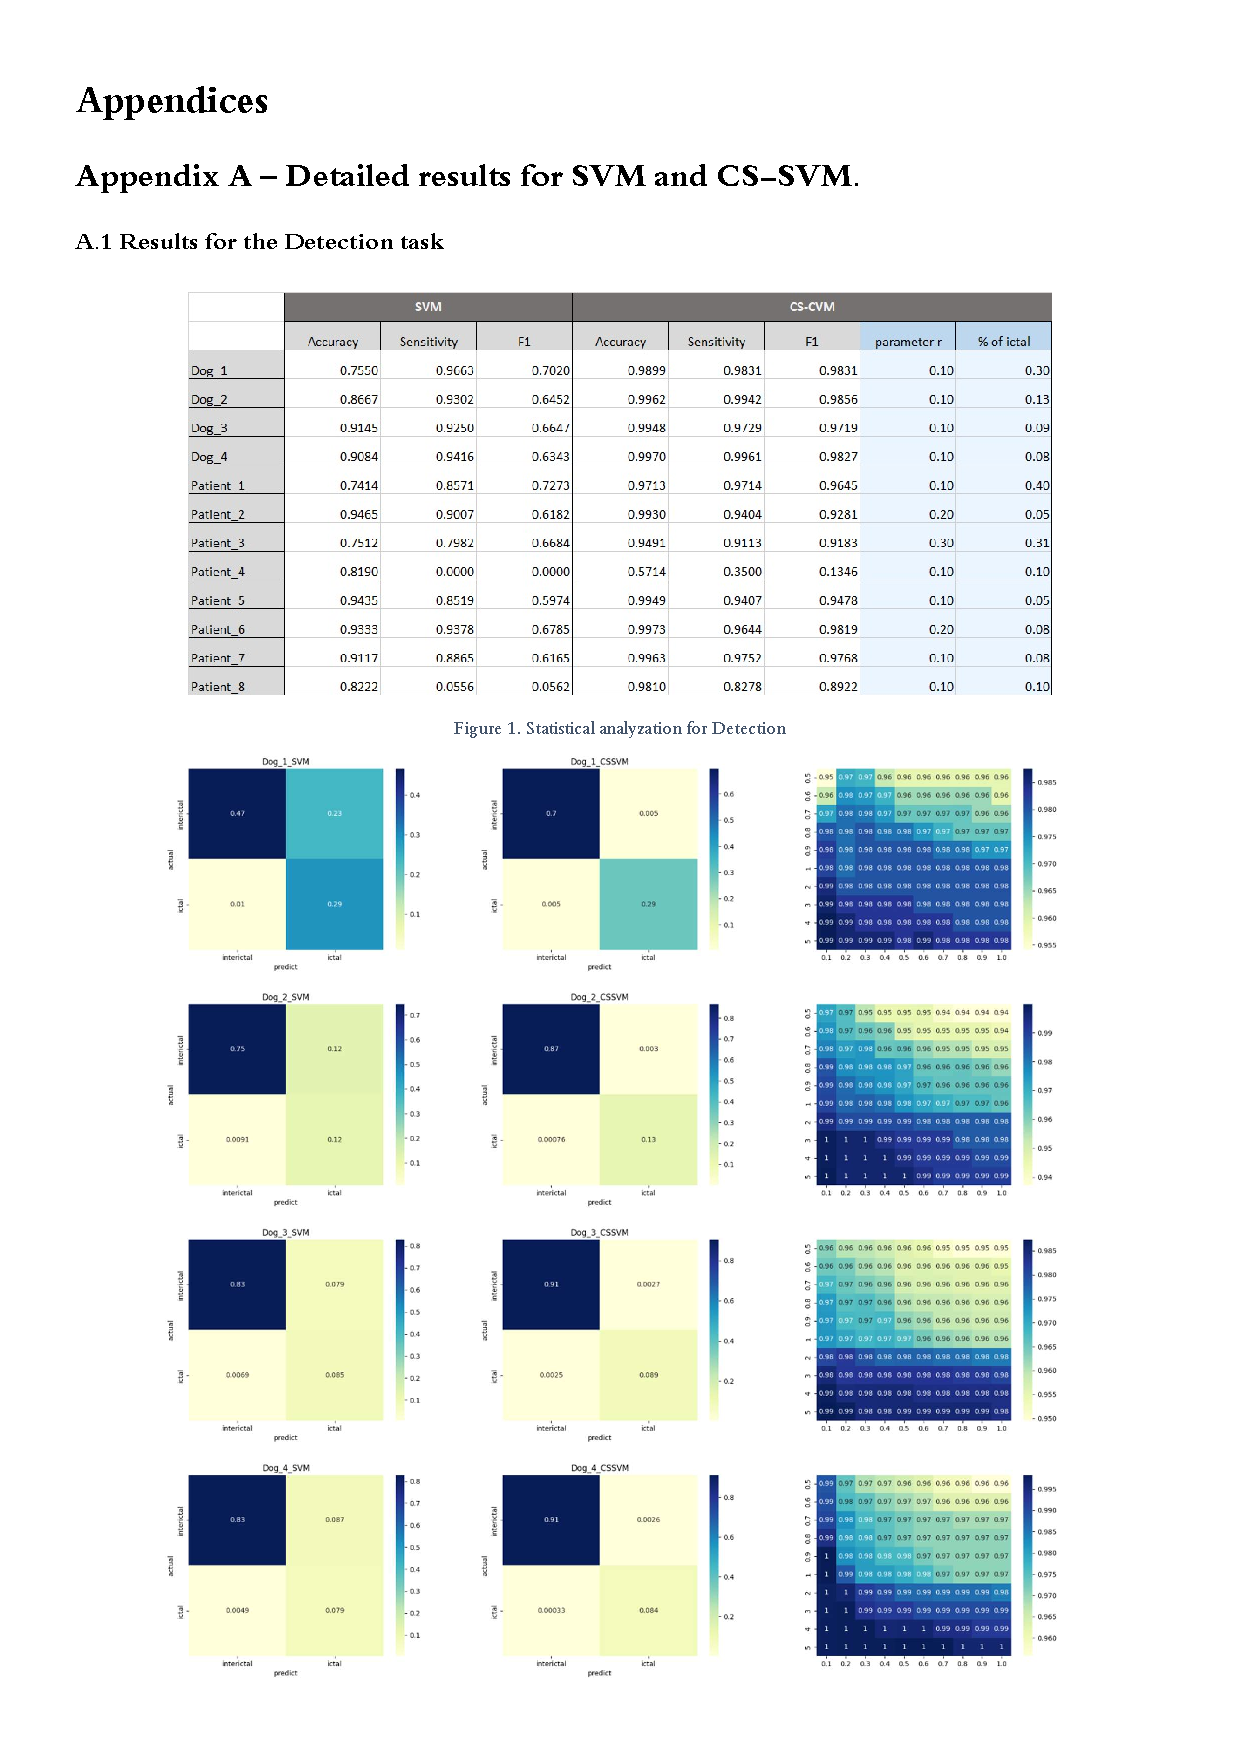
\includepdf[pages=1-5]{Appendice.pdf}
\end{document}